% Options for packages loaded elsewhere
\PassOptionsToPackage{unicode}{hyperref}
\PassOptionsToPackage{hyphens}{url}
\PassOptionsToPackage{dvipsnames,svgnames,x11names}{xcolor}
%
\documentclass[
  11pt,
]{article}

\usepackage{amsmath,amssymb}
\usepackage{iftex}
\ifPDFTeX
  \usepackage[T1]{fontenc}
  \usepackage[utf8]{inputenc}
  \usepackage{textcomp} % provide euro and other symbols
\else % if luatex or xetex
  \usepackage{unicode-math}
  \defaultfontfeatures{Scale=MatchLowercase}
  \defaultfontfeatures[\rmfamily]{Ligatures=TeX,Scale=1}
\fi
\usepackage{lmodern}
\ifPDFTeX\else  
    % xetex/luatex font selection
    \setmainfont[]{Aptos}
\fi
% Use upquote if available, for straight quotes in verbatim environments
\IfFileExists{upquote.sty}{\usepackage{upquote}}{}
\IfFileExists{microtype.sty}{% use microtype if available
  \usepackage[]{microtype}
  \UseMicrotypeSet[protrusion]{basicmath} % disable protrusion for tt fonts
}{}
\makeatletter
\@ifundefined{KOMAClassName}{% if non-KOMA class
  \IfFileExists{parskip.sty}{%
    \usepackage{parskip}
  }{% else
    \setlength{\parindent}{0pt}
    \setlength{\parskip}{6pt plus 2pt minus 1pt}}
}{% if KOMA class
  \KOMAoptions{parskip=half}}
\makeatother
\usepackage{xcolor}
\setlength{\emergencystretch}{3em} % prevent overfull lines
\setcounter{secnumdepth}{-\maxdimen} % remove section numbering
% Make \paragraph and \subparagraph free-standing
\makeatletter
\ifx\paragraph\undefined\else
  \let\oldparagraph\paragraph
  \renewcommand{\paragraph}{
    \@ifstar
      \xxxParagraphStar
      \xxxParagraphNoStar
  }
  \newcommand{\xxxParagraphStar}[1]{\oldparagraph*{#1}\mbox{}}
  \newcommand{\xxxParagraphNoStar}[1]{\oldparagraph{#1}\mbox{}}
\fi
\ifx\subparagraph\undefined\else
  \let\oldsubparagraph\subparagraph
  \renewcommand{\subparagraph}{
    \@ifstar
      \xxxSubParagraphStar
      \xxxSubParagraphNoStar
  }
  \newcommand{\xxxSubParagraphStar}[1]{\oldsubparagraph*{#1}\mbox{}}
  \newcommand{\xxxSubParagraphNoStar}[1]{\oldsubparagraph{#1}\mbox{}}
\fi
\makeatother


\providecommand{\tightlist}{%
  \setlength{\itemsep}{0pt}\setlength{\parskip}{0pt}}\usepackage{longtable,booktabs,array}
\usepackage{calc} % for calculating minipage widths
% Correct order of tables after \paragraph or \subparagraph
\usepackage{etoolbox}
\makeatletter
\patchcmd\longtable{\par}{\if@noskipsec\mbox{}\fi\par}{}{}
\makeatother
% Allow footnotes in longtable head/foot
\IfFileExists{footnotehyper.sty}{\usepackage{footnotehyper}}{\usepackage{footnote}}
\makesavenoteenv{longtable}
\usepackage{graphicx}
\makeatletter
\def\maxwidth{\ifdim\Gin@nat@width>\linewidth\linewidth\else\Gin@nat@width\fi}
\def\maxheight{\ifdim\Gin@nat@height>\textheight\textheight\else\Gin@nat@height\fi}
\makeatother
% Scale images if necessary, so that they will not overflow the page
% margins by default, and it is still possible to overwrite the defaults
% using explicit options in \includegraphics[width, height, ...]{}
\setkeys{Gin}{width=\maxwidth,height=\maxheight,keepaspectratio}
% Set default figure placement to htbp
\makeatletter
\def\fps@figure{htbp}
\makeatother

\usepackage{booktabs}
\usepackage{longtable}
\usepackage{array}
\usepackage{multirow}
\usepackage{wrapfig}
\usepackage{float}
\usepackage{colortbl}
\usepackage{pdflscape}
\usepackage{tabu}
\usepackage{threeparttable}
\usepackage{threeparttablex}
\usepackage[normalem]{ulem}
\usepackage{makecell}
\usepackage{xcolor}
\usepackage{pdfpages}
\usepackage{fontspec}
\usepackage[bottom]{footmisc}
\setmainfont{Aptos}[Path="C:/Users/ginow/AppData/Roaming/TinyTeX/texmf-dist/fonts/truetype/aptos/", Extension=".ttf"]
\usepackage{fancyhdr}
\pagestyle{fancy}
\fancyhf{}
\fancyhead[C]{\makebox[\textwidth]{\hspace*{-1cm}
\includegraphics[height=1.9cm]{../Logotipo ENADEL/encabezado_izquierda.png} \hfill 
\includegraphics[height=1.5cm]{../Logotipo ENADEL/encabezado_derecha.png} \hspace*{-2cm}}}
\fancyfoot[L]{Subsecretaría del Trabajo}
\cfoot{\thepage}
\setlength{\footskip}{10pt}
\setlength{\skip\footins}{15pt}
\setlength{\headheight}{3cm}
\setlength{\headsep}{0.5cm}
\renewcommand{\footrulewidth}{0pt}
\floatplacement{figure}{H}
\floatplacement{table}{H}
\usepackage{geometry}
\geometry{ left=3cm, right=3cm, top=2.5cm, bottom=2.5cm }
\usepackage{placeins}
\usepackage{ragged2e}
\usepackage{float}
\usepackage{setspace}
\renewcommand{\familydefault}{\sfdefault}
\AtBeginDocument{\renewcommand{\baselinestretch}{1.5}\justifying}
\usepackage{xcolor}
\usepackage{pagecolor}
\makeatletter
\@ifpackageloaded{caption}{}{\usepackage{caption}}
\AtBeginDocument{%
\ifdefined\contentsname
  \renewcommand*\contentsname{Tabla de contenidos}
\else
  \newcommand\contentsname{Tabla de contenidos}
\fi
\ifdefined\listfigurename
  \renewcommand*\listfigurename{Listado de Figuras}
\else
  \newcommand\listfigurename{Listado de Figuras}
\fi
\ifdefined\listtablename
  \renewcommand*\listtablename{Listado de Tablas}
\else
  \newcommand\listtablename{Listado de Tablas}
\fi
\ifdefined\figurename
  \renewcommand*\figurename{Figura}
\else
  \newcommand\figurename{Figura}
\fi
\ifdefined\tablename
  \renewcommand*\tablename{Tabla}
\else
  \newcommand\tablename{Tabla}
\fi
}
\@ifpackageloaded{float}{}{\usepackage{float}}
\floatstyle{ruled}
\@ifundefined{c@chapter}{\newfloat{codelisting}{h}{lop}}{\newfloat{codelisting}{h}{lop}[chapter]}
\floatname{codelisting}{Listado}
\newcommand*\listoflistings{\listof{codelisting}{Listado de Listados}}
\makeatother
\makeatletter
\makeatother
\makeatletter
\@ifpackageloaded{caption}{}{\usepackage{caption}}
\@ifpackageloaded{subcaption}{}{\usepackage{subcaption}}
\makeatother

\ifLuaTeX
\usepackage[bidi=basic]{babel}
\else
\usepackage[bidi=default]{babel}
\fi
\babelprovide[main,import]{spanish}
\ifPDFTeX
\else
\babelfont{rm}[]{Aptos}
\fi
% get rid of language-specific shorthands (see #6817):
\let\LanguageShortHands\languageshorthands
\def\languageshorthands#1{}
\ifLuaTeX
  \usepackage{selnolig}  % disable illegal ligatures
\fi
\usepackage{bookmark}

\IfFileExists{xurl.sty}{\usepackage{xurl}}{} % add URL line breaks if available
\urlstyle{same} % disable monospaced font for URLs
\hypersetup{
  pdflang={es},
  colorlinks=true,
  linkcolor={blue},
  filecolor={Maroon},
  citecolor={Blue},
  urlcolor={Blue},
  pdfcreator={LaTeX via pandoc}}


\author{}
\date{}

\begin{document}

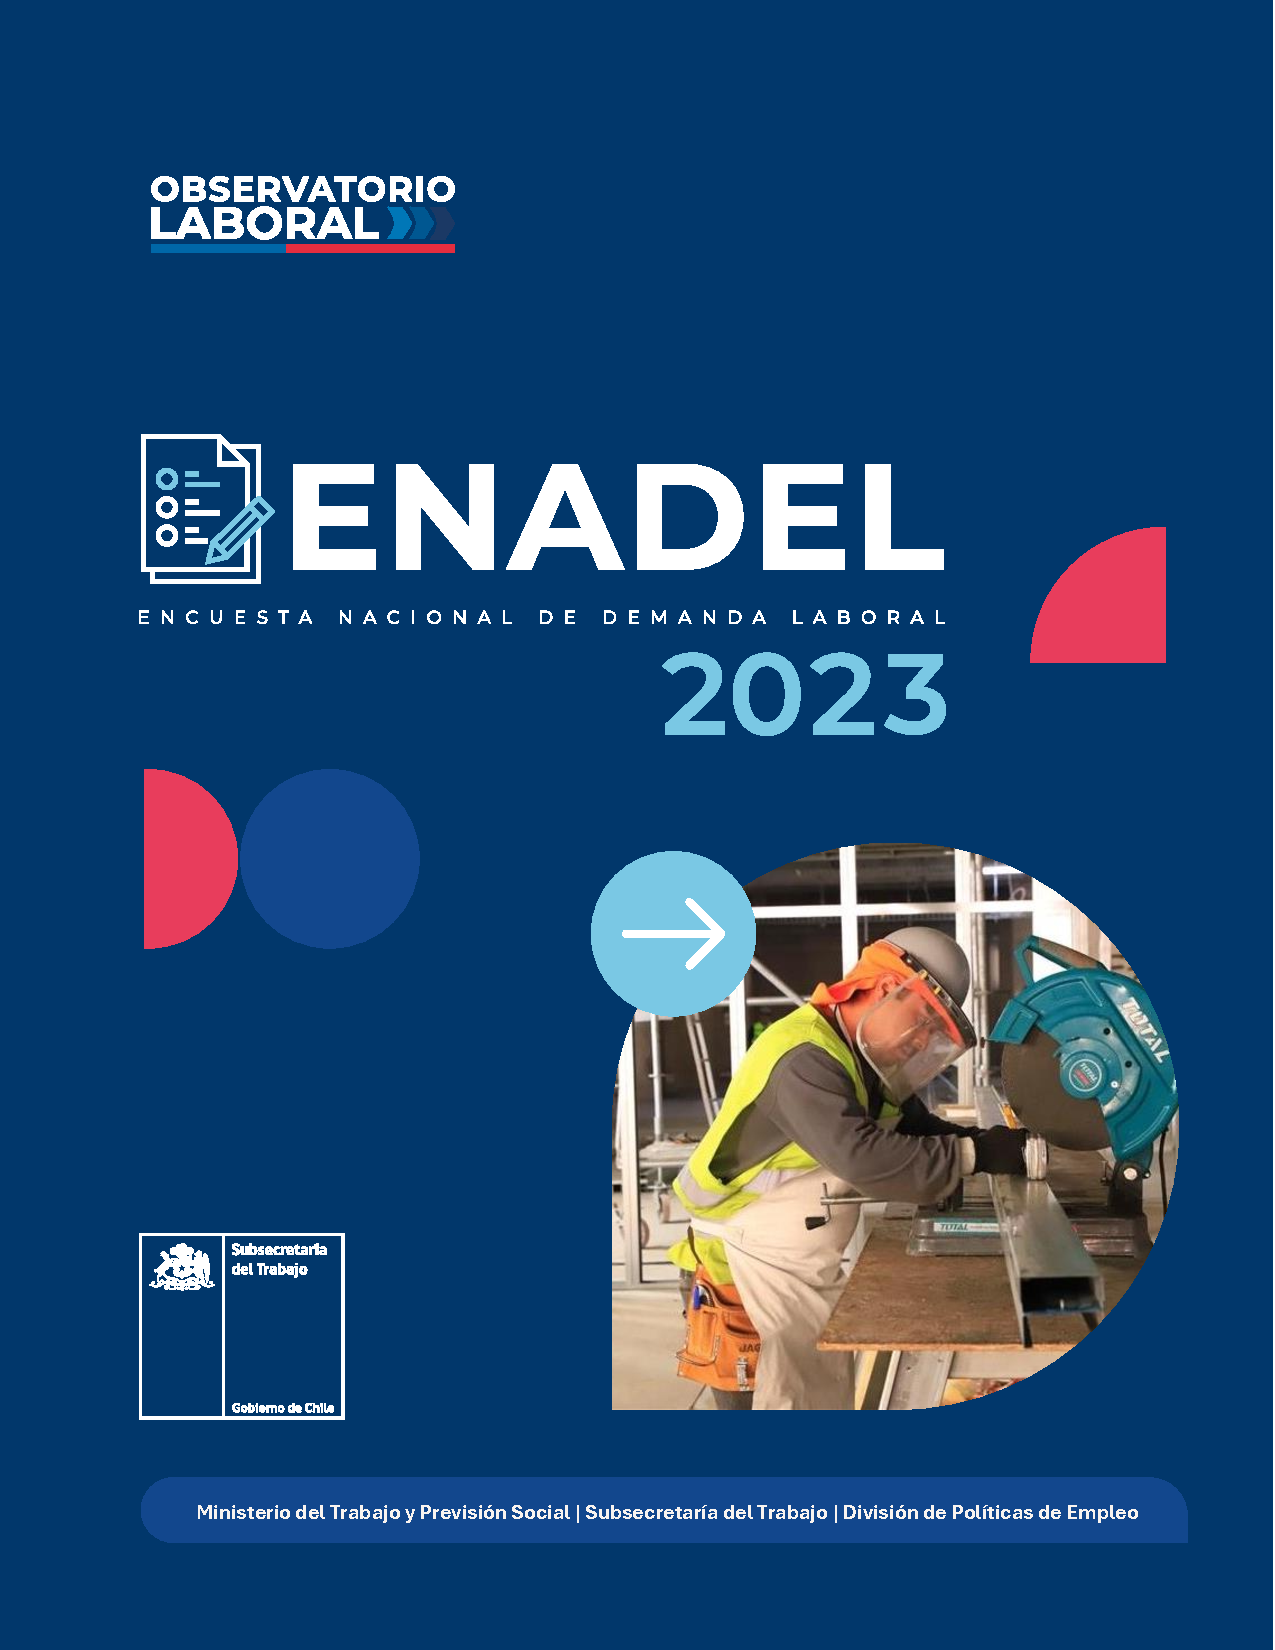
\includepdf[pages=-]{../Quarto/Portada/Portadas-Enadel-2023-1.pdf}


\newpage

\thispagestyle{empty}

\centering


\includegraphics[width=0.5\textwidth]{../Logotipo ENADEL/logotipo-ENADEL-2023.png}
\vspace{2cm}

\noindent Ministerio del Trabajo y Previsión Social

División de Políticas de Empleo\textbackslash{} Subsecretaría del
Trabajo

\justifying

El presente documento analiza los resultados de la Encuesta Nacional de
Demanda Laboral (ENADEL) 2023, que busca identificar y caracterizar el
capital humano requerido por las empresas de los distintos sectores
productivos del país, generando información sobre la demanda actual de
ocupaciones de las empresas, detectando requisitos y problemas de
contratación. Al igual que versiones anteriores de esta encuesta, se
puso el foco en dos sectores de actividad económica: Construcción y el
sector Agrícola.

\newpage
\renewcommand{\contentsname}{Índice} 
\tableofcontents

\newpage

\subsection{Descripción General: Empresas y
Trabajadores}\label{descripciuxf3n-general-empresas-y-trabajadores}

La muestra de ENADEL 2023 encuesta a 5.820 empresas que suman 485.256
trabajadores (a nivel muestral). Estas representan a 82.052 empresas y
5.611.196 trabajadores a nivel nacional. La Tabla~\ref{tbl-region}
muestra la distribución en las distintas regiones del país, dónde un
\text{53,6}\% de las empresas y un \text{65,6}\% de los trabajadores se
encuentran en la región Metropolitana.

\vspace{5mm}

\FloatBarrier

\begin{table}

\caption{\label{tbl-region}Resultados de la encuesta}

\centering{

\centering
\begin{tabular}{>{\raggedright\arraybackslash}p{6cm}>{\raggedright\arraybackslash}p{3cm}>{\raggedright\arraybackslash}p{3cm}}
\toprule
Región & \% Empresas & \% Trabajadores\\
\midrule
Arica y Parinacota & 0,7\% & 0,3\%\\
Tarapacá & 1,7\% & 1,1\%\\
Antofagasta & 2,6\% & 1,8\%\\
Atacama & 0,8\% & 0,5\%\\
Coquimbo & 2,8\% & 1,9\%\\
\addlinespace
Valparaíso & 9,1\% & 6,5\%\\
Metropolitana & 53,6\% & 65,6\%\\
O'Higgins & 5,1\% & 4,2\%\\
Maule & 1,5\% & 1\%\\
Ñuble & 6,7\% & 5\%\\
\addlinespace
Biobío & 1,3\% & 0,7\%\\
Araucanía & 4,6\% & 3,4\%\\
Los Ríos & 0,4\% & 0,3\%\\
Los Lagos & 1\% & 0,6\%\\
Aysén & 4,9\% & 4,7\%\\
\addlinespace
Magallanes & 3,3\% & 2,3\%\\
\bottomrule
\multicolumn{3}{l}{\rule{0pt}{1em}Fuente: Elaboración propia utilizando datos de ENADEL 2023, datos expandidos.}\\
\end{tabular}

}

\end{table}%

\FloatBarrier

La Figura~\ref{fig-combined} muestra el porcentaje de empresas y
trabajadores según tamaño de empresas, utilizando la clasificación por
número de trabajadores, cómo por volumen de venta. Con respecto a la
primera clasificación, el 74,6\% de las empresas tiene menos de 50
trabajadores --acumulando un 23,8\% del total-- y casi el 50\% de los
trabajadores están en empresas grandes --que corresponden a un 6,5\% del
total. Si se analiza según tamaño de ventas, más de la mitad de las
empresas tienen un volumen de venta de entre 2.400 y 24.999 UF
(``Pequeñas'') y más de un cuarto venden entre 25.000 y 100.000 UF al
año (``Mediana''). Sin embargo, casi un tercio de los trabajadores están
en empresas grandes (más de 100.000 UF).

\FloatBarrier

\begin{figure}[H]

\caption{\label{fig-combined}Gráfico combinado de resultados}

\centering{

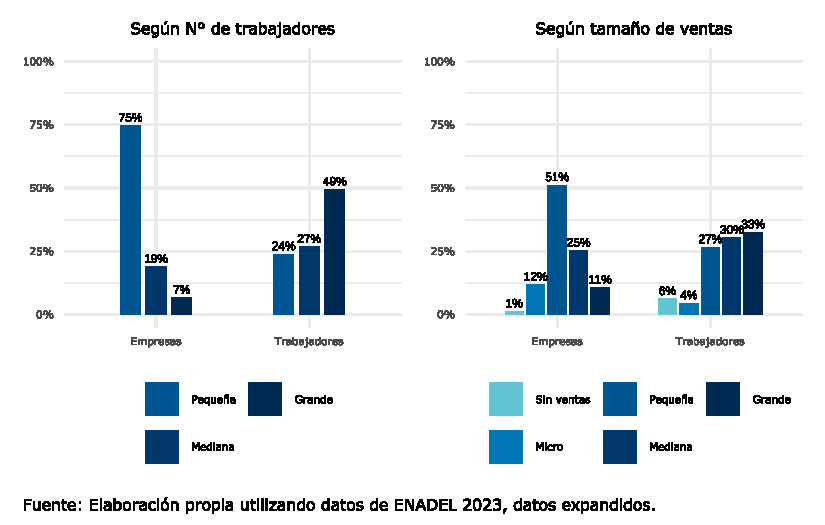
\includegraphics[width=1\textwidth,height=\textheight]{Reporte_files/figure-pdf/fig-combined-1.pdf}

}

\end{figure}%

\FloatBarrier

Al revisar la distribución por sector de actividad económica
Tabla~\ref{tbl-acteco} se tiene que una de cada cinco empresas pertenece
al sector de Comercio, seguido por el sector Construcción
(\text{15,5}\%) y el sector de Industrias Manufactureras (11,4\%). Con
respecto al volumen de trabajadores, el sector Comercio también lidera
(17,8\%) seguido por el sector Construcción (14,4\%) y el sector de
Servicios Administrativos y de Apoyo que, siendo sector intensivo en
trabajo, un 9,1\% de las empresas acumula el 13,5\% de trabajadores y
trabajadoras.

\FloatBarrier

\begin{table}

\caption{\label{tbl-acteco}Empresas y trabajadores según sector de
actividad económica}

\centering{

\centering
\begin{tabular}{>{\raggedright\arraybackslash}p{11cm}ll}
\toprule
Actividad Económica & \% Empresas & \% Trabajadores\\
\midrule
Comercio & 20,6\% & 17,8\%\\
Construcción & 15,5\% & 14,4\%\\
Servicios administrativos y de apoyo & 9,1\% & 13,5\%\\
Industria manufacturera & 11,4\% & 11,8\%\\
Actividades profesionales & 10,8\% & 11\%\\
\addlinespace
Silvoagropecuario & 8,6\% & 8,3\%\\
Transporte y almacenamiento & 7,6\% & 5,9\%\\
Administración pública & 0,7\% & 5,5\%\\
Alojamiento y de servicio de comidas & 6,8\% & 4\%\\
Información y comunicaciones & 3,2\% & 2,6\%\\
\addlinespace
Actividades inmobiliarias & 3\% & 2,6\%\\
Actividades financieras y de seguros & 1,9\% & 1,7\%\\
Pesca y acuicultura & 0,8\% & 0,9\%\\
\bottomrule
\multicolumn{3}{l}{\rule{0pt}{1em}Fuente: Elaboración propia utilizando datos de ENADEL 2023, datos expandidos.}\\
\end{tabular}

}

\end{table}%

\FloatBarrier

\subsection{Contratados en los últimos 12
meses}\label{contratados-en-los-uxfaltimos-12-meses}

El 87,1\% de las empresas declaró que sí contrató personas nuevas
durante los últimos 12 meses, mientras que el 12,9\% declara que no
contrató personas nuevas durante el mismo período. La
Tabla~\ref{tbl-contratos_totales} muestra la proporción de empresas,
según sector de actividad económica, que tuvieron contrataciones nuevas
durante los últimos 12 meses. El 98.9\% de las empresas del sector de
pesca y acuicultura respondieron afirmativamente, mientras que el sector
con menor proporción fue el de Actividades Inmobiliarias, dónde el
24,9\% de firmas no tuvieron contrataciones durante los últimos 12
meses.

\FloatBarrier

\begin{table}

\caption{\label{tbl-contratos_totales}Porcentaje de empresas que
contrataron en los últimos 12 meses por sector económico}

\centering{

\centering
\begin{tabular}{>{\raggedright\arraybackslash}p{11cm}ll}
\toprule
Actividad Económica & \% Si & \% No\\
\midrule
Actividades profesionales & 90,4\% & 9,6\%\\
Actividades financieras y de seguros & 83,9\% & 16,1\%\\
Actividades inmobiliarias & 75,1\% & 24,9\%\\
Administración pública & 90,3\% & 9,7\%\\
Alojamiento y de servicio de comidas & 92,9\% & 7,1\%\\
\addlinespace
Comercio & 84,8\% & 15,2\%\\
Construcción & 89,3\% & 10,7\%\\
Industria manufacturera & 87,3\% & 12,7\%\\
Información y comunicaciones & 90,3\% & 9,7\%\\
Servicios administrativos y de apoyo & 87,5\% & 12,5\%\\
\addlinespace
Silvoagropecuario & 83,6\% & 16,4\%\\
Pesca y acuicultura & 98,9\% & 1,1\%\\
Transporte y almacenamiento & 85\% & 15\%\\
Total & 87,6\% & 12,4\%\\
\bottomrule
\multicolumn{3}{l}{\rule{0pt}{1em}Fuente: Elaboración propia utilizando datos de ENADEL 2023, datos expandidos.}\\
\end{tabular}

}

\end{table}%

\FloatBarrier

\subsubsection{Contrataciones por
ocupación}\label{contrataciones-por-ocupaciuxf3n}

Se contrataron cargos\footnote{Contrataciones señaladas para los módulos
  de ``Directores y gerentes'', ``Jefatura/ADP'', ``Ocupaciones
  Elementales'' y ``Otros Cargos''.} nuevos en 354 ocupaciones
(representando a 1.206.992 contrataciones totales en los últimos 12
meses, cv = 6,8\%), sin embargo, la Tabla~\ref{tbl-contratados_u12} sólo
muestra aquellas para las cuáles el coeficiente de variación es menor a
20\%\footnote{La convención es considerar cómo robustas estimaciones con
  un cv menor al 15\%. Dado que estas son pocas, se presentan todas las
  ocupaciones con un cv menor a 20\%.}. Las ocupaciones con más
contratos en los últimos 12 meses fueron ``Obreros de explotaciones
agrícolas'', ``Auxiliares de aseo de oficinas, hoteles y otros
establecimientos'' y ``Vendedores y asistentes de venta de tiendas,
almacenes y puestos de mercado''.

\begin{table}

\caption{\label{tbl-contratados_u12}Contratados últimos 12 meses, por
ocupación.}

\centering{

\centering
\begin{tabular}{>{\raggedleft\arraybackslash}p{1.2cm}>{\raggedright\arraybackslash}p{11cm}rl}
\toprule
CIUO\_08 & Glosa & Contratados & cv\\
\midrule
9211 & Obreros de explotaciones agrícolas & 300480 & 19,2\%\\
9112 & Auxiliares de aseo de oficinas, hoteles y otros establecimientos & 71821 & 16,4\%\\
5223 & Vendedores y asistentes de venta de tiendas, almacenes y puestos de mercado & 23492 & 15,7\%\\
5414 & Guardias de seguridad & 17719 & 12,9\%\\
5131 & Garzones de mesa & 13484 & 10,4\%\\
\addlinespace
8332 & Conductores de camiones pesados y de alto tonelaje & 12410 & 9,5\%\\
5120 & Cocineros & 7623 & 14,7\%\\
3123 & Supervisores de la construcción & 5224 & 19,2\%\\
2243 & Ingenieros en prevención de riesgos y otros profesionales de la seguridad e higiene laboral y ambiental & 2971 & 19,2\%\\
8331 & Conductores de buses y trolebuses & 2968 & 16,6\%\\
\addlinespace
8350 & Tripulantes de cubierta de barco & 1639 & 18,7\%\\
\bottomrule
\multicolumn{4}{l}{\rule{0pt}{1em}Fuente: Elaboración propia utilizando datos de ENADEL 2023, datos expandidos.}\\
\end{tabular}

}

\end{table}%

\newpage

\subsubsection{Contrataciones por ocupación: Sector
Construcción}\label{contrataciones-por-ocupaciuxf3n-sector-construcciuxf3n}

En el módulo del sector Construcción se consulta sobre las
contrataciones de 25 cargos específicos, con un total de 365.712
contrataciones en los últimos 12 meses (cv=29,2\%). La
Tabla~\ref{tbl-contratados_u12_constru} muestra la proporción de
contratados por cargo, con respecto al total de este módulo. El cargo de
``Obreros y jornales'' es el que concentra la mayor cantidad de
contrataciones, seguido por ``Carpinteros'' y por ``Electricistas
(técnicos y/o maestros)''.

\begin{table}

\caption{\label{tbl-contratados_u12_constru}Proporción de contrataciones
por ocupación, sector construcción.}

\centering{

\centering
\begin{tabular}{>{\raggedright\arraybackslash}p{12cm}l}
\toprule
Cargo Construcción & \%\\
\midrule
Obreros y jornales & 23,2\%\\
Carpinteros & 12,2\%\\
Electricistas (técnicos y/o maestros) & 11,5\%\\
Otros maestros de primera y segunda & 9,7\%\\
Albañiles & 7\%\\
\addlinespace
Enfierradores & 4\%\\
Concreteros & 3,7\%\\
Operadores de maquinaria pesada & 3,2\%\\
Pintores & 3,1\%\\
Operadores de maquinaria liviana & 3\%\\
\addlinespace
Ingenieros, prevencionistas, arqueólogos, otros profesionales & 2,6\%\\
Baldoseros y ceramistas & 2,6\%\\
Soldadores & 2,4\%\\
Capataces & 2,3\%\\
Encargados de Obra & 2,1\%\\
\addlinespace
Electrónicos, electromecánicos e instrumentistas & 2,1\%\\
Mecánicos & 1,6\%\\
Trazadores & 1,1\%\\
Bodegueros y cardcheckers & 1\%\\
Sanitarios y gásfiteres & 0,4\%\\
\addlinespace
Instaladores de gas & 0,4\%\\
Operadores planta asfalto y áridos & 0,3\%\\
Laboratoristas & 0,2\%\\
Tuberos y peradores de termofusión & 0,2\%\\
Buzos & 0\%\\
\bottomrule
\multicolumn{2}{l}{\rule{0pt}{1em}Fuente: Elaboración propia utilizando datos de ENADEL 2023, datos expandidos.}\\
\end{tabular}

}

\end{table}%

\subsubsection{Contrataciones por ocupación: Sector
Agrícola}\label{contrataciones-por-ocupaciuxf3n-sector-agruxedcola}

En el módulo del sector Agrícola se consulta sobre las contrataciones de
15 cargos específicos, con un total de 321.395 contrataciones en los
últimos 12 meses (cv=21,6\%), cuya distribución en los distintos cargos
se muestra en la Tabla~\ref{tbl-contratados_u12_agricola}. Las
ocupaciones de ``Obrero agrícola de cosecha'' y ``Obrero agrícola de
packing frutícola, bodega, estabilización, embotellado'' son las que
lideran las contrataciones durante los últimos 12 meses.

\begin{table}

\caption{\label{tbl-contratados_u12_agricola}Proporción de
contrataciones por ocupación, sector agrícola}

\centering{

\centering
\begin{tabular}{ll}
\toprule
Cargo Agrícola & \%\\
\midrule
Obrero agrícola de cosecha & 37,6\%\\
Obrero agrícola de packing frutícola, bodega, estabilización, embotellado & 37,4\%\\
Obrero agrícola de poda, raleo & 11,3\%\\
Obrero agrícola de siembra, viveros & 3,7\%\\
Obrero agrícola de riego, aplicación de agroquímicos & 3,2\%\\
\addlinespace
Obrero forestal de cosecha & 1,9\%\\
Obrero agrícola de almácigos & 1,7\%\\
Obrero forestal de siembra & 1,2\%\\
Obrero pecuario de crianza, alimentación, pastoreo & 0,8\%\\
Obrero agroindustrial gestión de cría y engorda & 0,6\%\\
\addlinespace
Obrero forestal en labores de aserrador & 0,3\%\\
Obrero pecuario de ordeña & 0,2\%\\
Obrero agrícola de manejo reproductivo y sanitario & 0\%\\
Obrero agroindustrial en matadero & 0\%\\
Obrero agroindustrial limpieza, control plagas y enfermedades & 0\%\\
\bottomrule
\multicolumn{2}{l}{\rule{0pt}{1em}Fuente: Elaboración propia utilizando datos de ENADEL 2023, datos expandidos.}\\
\end{tabular}

}

\end{table}%

\subsection{Vacantes en los últimos 12
meses}\label{vacantes-en-los-uxfaltimos-12-meses}

El 72,05\% de las empresas declaró que sí tuvo vacantes no llenadas
durante los últimos 12 meses, mientras que el 27,95\% declara que no
tuvo vacantes no llenadas durante el mismo período.

La Tabla~\ref{tbl-vacantes_totales_sector} muestra la proporción de
empresas, según sector de actividad económica, que tuvieron vacantes no
llenadas durante los últimos 12 meses. El 89.5\% de las empresas del
sector de ``Información y comunicaciones'' tuvieron vacantes no
llenadas, lo mismo ocurre con el 87.7\% de las personas jurídicas del
sector de ``Administración pública'' y el 80.2\% del sector de
``Actividades profesionales''. Por otro lado, el sector de actividad
económica con un menor porcentaje de empresas que tuvieron vacantes no
llenadas fue el ``Silvoagropecuario''.

\begin{table}

\caption{\label{tbl-vacantes_totales_sector}Porcentaje de empresas con
vacantes no cubiertas}

\centering{

\centering
\begin{tabular}{>{\raggedright\arraybackslash}p{10cm}ll}
\toprule
Sector Actividad Económica & \% Sí & \% No\\
\midrule
Información y comunicaciones & 89,5\% & 10,5\%\\
Administración pública & 87,7\% & 12,3\%\\
Actividades profesionales & 80,2\% & 19,8\%\\
Alojamiento y de servicio de comidas & 78,3\% & 21,7\%\\
Transporte y almacenamiento & 78,3\% & 21,7\%\\
\addlinespace
Servicios administrativos y de apoyo & 76,4\% & 23,6\%\\
Industria manufacturera & 73,7\% & 26,3\%\\
Comercio & 72,3\% & 27,7\%\\
Construcción & 67,8\% & 32,2\%\\
Actividades financieras y de seguros & 67,6\% & 32,4\%\\
\addlinespace
Actividades inmobiliarias & 63\% & 37\%\\
Pesca y acuicultura & 61,7\% & 38,3\%\\
Silvoagropecuario & 49,4\% & 50,6\%\\
\bottomrule
\multicolumn{3}{l}{\rule{0pt}{1em}Fuente: Elaboración propia utilizando datos de ENADEL 2023, datos expandidos.}\\
\end{tabular}

}

\end{table}%

Durante el resto de esta sección se hará referencia a las ocupaciones
que tengan vacantes sin llenar durante los últimos 12 meses como
\textbf{ocupaciones de difícil cobertura}.

\newpage

\subsubsection{Ocupaciones de difícil
cobertura}\label{ocupaciones-de-difuxedcil-cobertura}

Se declararon vacantes\footnote{Vacantes señaladas para los módulos de
  ``Directores y gerentes'', ``Jefatura/ADP'', ``Ocupaciones
  Elementales'' y ``Otros Cargos''.} sin llenar en 215 ocupaciones
(68.365 vacantes, cv=12,3\%), sin embargo, la
Tabla~\ref{tbl-cuadro8_odc} sólo muestra aquellas para las cuáles el
coeficiente de variación es menor a 40\%\footnote{La convención es
  considerar cómo robustas estimaciones con un cv menor al 15\%. Dado
  que esto no se cumple, se presentan todas las ocupaciones con un cv
  menor a 40\%.}. La tabla completa con todas las ocupaciones de difícil
cobertura se puede encontrar en el \textbf{Apéndice A: Ocupaciones de
Difícil Cobertura}.

\begin{table}

\caption{\label{tbl-cuadro8_odc}Ocupaciones de difícil cobertura, ENADEL
2023.}

\centering{

\centering
\begin{tabular}{>{\raggedleft\arraybackslash}p{1.2cm}>{\raggedright\arraybackslash}p{11cm}rl}
\toprule
CIUO 08 & Glosa & Vacantes & cv\\
\midrule
9211 & Obreros de explotaciones agrícolas & 15147 & 36,5\%\\
9112 & Auxiliares de aseo de oficinas, hoteles y otros establecimientos & 1864 & 23,9\%\\
5414 & Guardias de seguridad & 1727 & 30,4\%\\
8322 & Conductores de automóviles, taxis y camionetas & 1503 & 36,9\%\\
5223 & Vendedores y asistentes de venta de tiendas, almacenes y puestos de mercado & 1086 & 37,1\%\\
\addlinespace
8332 & Conductores de camiones pesados y de alto tonelaje & 997 & 26,1\%\\
7233 & Mecánicos y reparadores de máquinas agrícolas e industriales & 499 & 31,3\%\\
8343 & Operadores de grúas y aparatos elevadores & 489 & 28,8\%\\
7512 & Panaderos, pasteleros y confiteros & 171 & 31,2\%\\
2142 & Ingenieros civiles, ingenieros en construcción y constructores civiles & 92 & 38,3\%\\
\addlinespace
8342 & Operadores de máquinas de movimiento de tierras & 79 & 36,2\%\\
\bottomrule
\multicolumn{4}{l}{\rule{0pt}{1em}Fuente: Elaboración propia utilizando datos de ENADEL 2023, datos expandidos.}\\
\end{tabular}

}

\end{table}%

La ocupación más demandadas que tiene difícil cobertura es ``Obreros de
explotaciones agrícolas'', con más de 14 mil vacantes; seguido de lejos
por ``Auxiliares de aseo de oficinas, hoteles y otros
establecimientos'', ``Guardias de seguridad'' y ``Conductores de
automóviles, taxis y camionetas'', con 1864, 1727 y 1503 vacantes,
respectivamente.

La Tabla~\ref{tbl-vacantes_region} muestra la ocupación de difícil
cobertura con mayor cantidad de vacantes por región dónde, si bien se
confirma la prevalencia de ``Obreros de explotaciones agrícolas'' en 7
regiones, también saltan a la vista otros patrones como la demanda del
rubro de la construcción hacia el norte y de la industria manufacturera
en el Maule y la Araucanía.

\begin{table}

\caption{\label{tbl-vacantes_region}Ocupación de difícil cobertura con
mayor cantidad de vacantes, por región.}

\centering{

\centering
\begin{tabular}{l>{\raggedright\arraybackslash}p{7cm}rr}
\toprule
Región & Ocupación & CIUO 08 & Vacantes\\
\midrule
Arica y Parinacota & Obreros de la construcción de edificios & 9313 & 91\\
Tarapacá & Otros operarios de la construcción (obra gruesa) no clasificados previamente & 7119 & 112\\
Antofagasta & Soldadores y oxicortadores & 7212 & 66\\
Atacama & Obreros de explotaciones agrícolas & 9211 & 2943\\
Coquimbo & Cocineros de comida rápida & 9411 & 236\\
\addlinespace
Valparaíso & Obreros de explotaciones agrícolas & 9211 & 1076\\
Metropolitana & Obreros de explotaciones agrícolas & 9211 & 3376\\
O'Higgins & Secretarios generales & 4120 & 269\\
Maule & Obreros de la industria manufacturera no clasificados previamente & 9329 & 93\\
Ñuble & Agricultores y trabajadores calificados de cultivos extensivos & 6111 & 151\\
\addlinespace
Biobío & Obreros de explotaciones agrícolas & 9211 & 27\\
Araucanía & Operadores de máquinas de preparación de fibras, hilado y devanado & 8151 & 32\\
Los Ríos & Obreros de explotaciones agrícolas & 9211 & 7397\\
Los Lagos & Obreros de explotaciones agrícolas & 9211 & 49\\
Aysén & Auxiliares de aseo de oficinas, hoteles y otros establecimientos & 9112 & 41\\
\addlinespace
Magallanes & Obreros de explotaciones agrícolas & 9211 & 217\\
\bottomrule
\multicolumn{4}{l}{\rule{0pt}{1em}Fuente: Elaboración propia utilizando datos de ENADEL 2023, datos expandidos.}\\
\end{tabular}

}

\end{table}%

Al indagar según el tamaño de empresa (Tabla~\ref{tbl-vacantes_tamano}),
``Obreros de explotaciones agrícolas'' prevalece en las empresas
pequeñas (tanto por número de trabajadores como por tamaño de venta) y
``Empacadores manuales'' en las empresas con más de 200 trabajadores y
en aquellas con ventas entre 25 y 100 mil UF. La ocupación
``Especialistas en políticas y servicios de personal'' es la más difícil
de cubrir en empresas de entre 50 y 199 trabajadores (mediana) y en
aquellas que tienen ventas superiores a las 10 mil UF.

\begin{table}

\caption{\label{tbl-vacantes_tamano}Ocupación de difícil cobertura con
mayor cantidad de vacantes por tamaño de empresa.}

\centering{

\centering\centering
\resizebox{\ifdim\width>\linewidth\linewidth\else\width\fi}{!}{
\begin{tabular}{>{\raggedright\arraybackslash}p{4cm}l>{\raggedright\arraybackslash}p{5cm}>{\raggedleft\arraybackslash}p{2cm}>{\raggedleft\arraybackslash}p{2cm}}
\toprule
Categoría & Tamaño Empresa & Ocupación & CIUO 08 & Vacantes\\
\midrule
\addlinespace[0.3em]
\multicolumn{5}{l}{\textbf{\textbf{Según n° de trabajadores}}}\\
\hspace{1em}\textbf{} & Pequeña (<50) & Obreros de explotaciones agrícolas & 9211 & 12571\\
\hspace{1em}\textbf{} & Mediana (50-199) & Especialistas en políticas y servicios de personal & 2423 & 2459\\
\hspace{1em}\textbf{} & Grande (>=200) & Empacadores manuales & 9321 & 1547\\
\addlinespace[0.3em]
\multicolumn{5}{l}{\textbf{\textbf{Según ventas}}}\\
\hspace{1em}\textbf{} & Sin ventas & Otro personal de los servicios de protección no clasificados previamente & 5419 & 146\\
\hspace{1em}\textbf{} & Micro (< 2.400 UF) & Conductores de camiones pesados y de alto tonelaje & 8332 & 219\\
\hspace{1em}\textbf{} & Pequeña (2.400-25.000 UF) & Obreros de explotaciones agrícolas & 9211 & 14374\\
\hspace{1em}\textbf{} & Mediana (25.000-100.000 UF) & Empacadores manuales & 9321 & 1778\\
\hspace{1em}\textbf{} & Grande (>100.000 UF) & Especialistas en políticas y servicios de personal & 2423 & 2459\\
\bottomrule
\multicolumn{5}{l}{\rule{0pt}{1em}Fuente: Elaboración propia utilizando datos de ENADEL 2023, datos expandidos.}\\
\end{tabular}}

}

\end{table}%

Al analizar las ocupaciones de difícil cobertura según el sector de
actividad económica, como se muestra en la
Tabla~\ref{tbl-vacantes_sector}, se vuelve a confirmar la dificultad
para llenar vacantes de ``Obreros de explotaciones agrícolas'', pero
también surgen otras ocupaciones relevantes como ``Obreros de
explotaciones agrícolas'' ``Vendedores y asistentes de venta de tiendas,
almacenes y puestos de mercado'' que es la ocupación con más vacantes
sin llenar en los sectores de ``Servicios administrativos y de apoyo'' y
``Transporte y almacenamiento''.

\begin{table}

\caption{\label{tbl-vacantes_sector}Ocupación de difícil cobertura con
mayor cantidad de vacantes por sector de actividad económica.}

\centering{

\centering
\begin{tabular}{>{\raggedright\arraybackslash}p{6cm}>{\raggedright\arraybackslash}p{6cm}>{\raggedleft\arraybackslash}p{1.3cm}>{\raggedleft\arraybackslash}p{1.3cm}}
\toprule
Sector Actividad Económica & Ocupación & CIUO 08 & Vacantes\\
\midrule
Silvoagropecuario & Obreros de explotaciones agrícolas & 9211 & 8654\\
Servicios administrativos y de apoyo & Obreros de explotaciones agrícolas & 9211 & 5755\\
Actividades profesionales & Especialistas en políticas y servicios de personal & 2423 & 2459\\
Alojamiento y de servicio de comidas & Ayudantes de cocina & 9412 & 1380\\
Construcción & Soldadores y oxicortadores & 7212 & 1377\\
\addlinespace
Transporte y almacenamiento & Obreros de carga & 9333 & 974\\
Comercio & Vendedores y asistentes de venta de tiendas, almacenes y puestos de mercado & 5223 & 882\\
Industria manufacturera & Obreros de la industria manufacturera no clasificados previamente & 9329 & 877\\
Información y comunicaciones & Instaladores y reparadores en tecnología de la información y las comunicaciones & 7422 & 340\\
Administración pública & Otro personal de los servicios de protección no clasificados previamente & 5419 & 146\\
\addlinespace
Actividades financieras y de seguros & Vendedores y asistentes de venta de tiendas, almacenes y puestos de mercado & 5223 & 43\\
Pesca y acuicultura & Carniceros y pescaderos & 7511 & 27\\
Actividades inmobiliarias & Personal de pompas fúnebres y embalsamadores & 5163 & 17\\
\bottomrule
\multicolumn{4}{l}{\rule{0pt}{1em}Fuente: Elaboración propia utilizando datos de ENADEL 2023, datos expandidos.}\\
\end{tabular}

}

\end{table}%

Nota: para seleccionar la ocupación de difícil cobertura con mayor
cantidad de vacantes sólo se tomó en cuenta la magnitud de la
estimación, sin considerar indicadores de robustez como el coeficiente
de variación. \newpage

\subsubsection{Ocupaciones de Difícil Cobertura: Sector
Construcción}\label{ocupaciones-de-difuxedcil-cobertura-sector-construcciuxf3n}

La Tabla~\ref{tbl-vacantes_constru} muestra todos los cargos del sector
Construcción sobre los que se consulta en la encuesta, indicando el
número de vacantes, el porcentaje que estas representan del total, y el
coeficiente de variación. Se muestran todas las vacantes independiente
de la robustez estadística de la estimación.

La ocupación de ``Obreros y jornales'' es la más demandada, con 1271
vacantes, seguida de ``Carpinteros'' con 495 vacantes y ``Soldadores''
con 406 vacantes.

\begin{table}

\caption{\label{tbl-vacantes_constru}Ocupaciones de difícil cobertura,
sector construcción.}

\centering{

\centering
\begin{tabular}{>{\raggedright\arraybackslash}p{9cm}rll}
\toprule
Cargo Construcción & Vacantes & \% del total & CV\\
\midrule
Obreros y jornales & 1271 & 39,5\% & 45,5\%\\
Carpinteros & 495 & 15,4\% & 52,1\%\\
Soldadores & 406 & 12,6\% & 82,7\%\\
Otros maestros de primera y segunda & 184 & 5,7\% & 90,5\%\\
Ingenieros, prevencionistas, arqueólogos, otros profesionales & 137 & 4,3\% & 53,7\%\\
\addlinespace
Pintores & 131 & 4,1\% & 59,3\%\\
Enfierradores & 119 & 3,7\% & 57,7\%\\
Albañiles & 101 & 3,1\% & 44,1\%\\
Capataces & 99 & 3,1\% & 51,1\%\\
Encargados de Obra & 63 & 2\% & 50,4\%\\
\addlinespace
Electrónicos, electromecánicos e instrumentistas & 59 & 1,8\% & 60,3\%\\
Baldoseros y ceramistas & 54 & 1,7\% & 78,2\%\\
Electricistas (técnicos y/o maestros) & 42 & 1,3\% & 47,4\%\\
Operadores de maquinaria pesada & 34 & 1\% & 77\%\\
Bodegueros y cardcheckers & 12 & 0,4\% & 71,6\%\\
\addlinespace
Mecánicos & 6 & 0,2\% & 100\%\\
Laboratoristas & 4 & 0,1\% & 100\%\\
Sanitarios y gásfiteres & 3 & 0,1\% & 100\%\\
Total & 3220 & 100\% & NA\%\\
\bottomrule
\multicolumn{4}{l}{\rule{0pt}{1em}Fuente: Elaboración propia utilizando datos de ENADEL 2023, datos expandidos.}\\
\end{tabular}

}

\end{table}%

\newpage

\subsubsection{Ocupaciones de Difícil Cobertura: Sector
Agrícola}\label{ocupaciones-de-difuxedcil-cobertura-sector-agruxedcola}

La Tabla~\ref{tbl-vacantes_agro} muestra todos los cargos del sector
Agrícola sobre los que se consulta en la encuesta, indicando el número
de vacantes, el porcentaje que estas representan del total, y el
coeficiente de variación. Se muestran todas las vacantes independiente
de la robustez estadística de la estimación.

El cargo ``Obrero agrícola de poda, raleo'' es el más demandado, con
``2234'' vacantes, el segundo cargo más demandado es ``Obrero agrícola
de cosecha'' con 1921 vacantes y `` Obrero agrícola de riego, aplicación
de agroquímicos'' es el tercer cargo más demandado con 1597 vacantes.

\begin{table}

\caption{\label{tbl-vacantes_agro}Ocupaciones de difícil cobertura,
sector agrícola.}

\centering{

\centering
\begin{tabular}{>{\raggedright\arraybackslash}p{7cm}rll}
\toprule
Cargo Agrícola & Vacantes & \% del total & CV\\
\midrule
Obrero agrícola de poda, raleo & 2234 & 21\% & 70\%\\
Obrero agrícola de cosecha & 1921 & 18,1\% & 80\%\\
Obrero agrícola de riego, aplicación de agroquímicos & 1597 & 15\% & 93\%\\
Obrero agrícola de siembra, viveros & 1488 & 14\% & 100\%\\
Obrero agrícola de packing frutícola, bodega, estabilización, embotellado & 1488 & 14\% & 84\%\\
\addlinespace
Obrero agrícola de almácigos & 1488 & 14\% & 100\%\\
Obrero forestal de siembra & 196 & 1,8\% & 100\%\\
Obrero forestal de cosecha & 173 & 1,6\% & 82\%\\
Obrero pecuario de ordeña & 41 & 0,4\% & 100\%\\
Total & 10626 & 100\% & NA\%\\
\bottomrule
\multicolumn{4}{l}{\rule{0pt}{1em}Fuente: Elaboración propia utilizando datos de ENADEL 2023, datos expandidos.}\\
\end{tabular}

}

\end{table}%

Al comparar los sectores agrícola y construcción, se puede notar que el
primer sector tiene una mayor dificultad para llenar sus vacantes:
mientras en el sector construcción las vacantes difíciles de llenar
equivalen al 0,88\% del total de contrataciones en los últimos 12 meses;
en el sector agrícola equivalen al 3,3\% de las contrataciones.

\newpage

\subsection{Dificultades para la
contratación}\label{dificultades-para-la-contrataciuxf3n}

El 20,6\% de las empresas declaró tener alguna dificultad durante el
proceso de contratación para llenar las vacantes disponibles\footnote{Se
  incluyen todas las vacantes para todos los cargos: módulos de
  ``Directores y gerentes'', ``Jefatura/ADP'', ``Ocupaciones
  Elementales'' y ``Otros Cargos''; Construcción y Agrícola.}. La
Tabla~\ref{tbl-dificultad_tot} muestra la proporción de respuestas para
la primera dificultad mencionada y para el total. Del total de
respuestas, la dificultad señalada más frecuentemente es ``Condiciones
laborales no aceptadas'' (16.6 \%), seguida de ``Falta de postulantes''
(14.8 \%) y Rotación laboral'' (12.9 \%).

\begin{table}

\caption{\label{tbl-dificultad_tot}Dificultades principales de
contratación.}

\centering{

\centering
\begin{tabular}{>{\raggedright\arraybackslash}p{5cm}>{\raggedright\arraybackslash}p{3cm}>{\raggedright\arraybackslash}p{3cm}}
\toprule
Primera dificultad & \% de 1ra dificultad & \% del total\\
\midrule
Condiciones laborales no aceptadas & 15,5\% & 16,6\%\\
Falta de postulantes & 15\% & 14,8\%\\
Rotación laboral & 13,9\% & 12,9\%\\
Candidatos sin competencias técnicas requeridas & 17\% & 12,5\%\\
Remuneración ofrecida no aceptada & 12,1\% & 12,3\%\\
\addlinespace
Candidatos sin la experiencia mínima requerida & 8,2\% & 10\%\\
Otra dificultad & 5,6\% & 7,6\%\\
Candidatos sin competencias socioemocionales requeridas & 6,6\% & 7\%\\
Candidatos sin licencias, certificaciones o requisitos legales & 5,4\% & 4,8\%\\
Candidatos sin nivel educacional requerido & 0,7\% & 1,5\%\\
\bottomrule
\multicolumn{3}{l}{\rule{0pt}{1em}Fuente: Elaboración propia utilizando datos de ENADEL 2023, datos expandidos.}\\
\end{tabular}

}

\end{table}%

\subsubsection{Dificultades para la contratación: Sector
Construcción}\label{dificultades-para-la-contrataciuxf3n-sector-construcciuxf3n}

Tabla~\ref{tbl-dificultad_constru} muestra que, al considerar el total
de menciones, ``Remuneración ofrecida no aceptada'' (22.4 \%), fue la
dificultad más mencionada, seguida de ``Condiciones laborales no
aceptadas'' (20.4 \%) y Falta de postulantes'' (15.9 \%).

\begin{table}

\caption{\label{tbl-dificultad_constru}Dificultades principales de
contratación, ocupaciones del sector Construcción.}

\centering{

\centering
\begin{tabular}{>{\raggedright\arraybackslash}p{5cm}>{\raggedright\arraybackslash}p{3cm}>{\raggedright\arraybackslash}p{3cm}}
\toprule
Primera dificultad & \% de 1ra dificultad & \% del total\\
\midrule
Remuneración ofrecida no aceptada & 29,8\% & 22,4\%\\
Condiciones laborales no aceptadas & 8,4\% & 20,4\%\\
Falta de postulantes & 22\% & 15,9\%\\
Rotación laboral & 10\% & 14,7\%\\
Candidatos sin la experiencia mínima requerida & 7,7\% & 7,6\%\\
\addlinespace
Candidatos sin licencias, certificaciones o requisitos legales & 10,4\% & 5,9\%\\
Candidatos sin competencias técnicas requeridas & 7,8\% & 5,7\%\\
Candidatos sin nivel educacional requerido & 0,7\% & 3,8\%\\
Candidatos sin competencias socioemocionales requeridas & 2,9\% & 2,8\%\\
Otra dificultad & 0,2\% & 0,8\%\\
\bottomrule
\multicolumn{3}{l}{\rule{0pt}{1em}Fuente: Elaboración propia utilizando datos de ENADEL 2023, datos expandidos.}\\
\end{tabular}

}

\end{table}%

\subsubsection{Dificultades para la contratación: Sector
Agrícola}\label{dificultades-para-la-contrataciuxf3n-sector-agruxedcola}

El 17,6\% de las empresas consultadas sobre ocupaciones del sector
Agrícola declararon tener alguna dificultad durante el proceso de
contratación. La Tabla~\ref{tbl-dificultad_agro} indica que las tres
dificultades más mencionadas son ``Condiciones laborales no aceptadas''
(31.1 \%), ``Rotación laboral'' (20.9 \%) y Falta de postulantes'' (19.1
\%).

\begin{table}

\caption{\label{tbl-dificultad_agro}Dificultades principales de
contratación, ocupaciones del sector Construcción.}

\centering{

\centering
\begin{tabular}{>{\raggedright\arraybackslash}p{5cm}>{\raggedright\arraybackslash}p{3cm}>{\raggedright\arraybackslash}p{3cm}}
\toprule
Primera dificultad & \% de 1ra dificultad & \% del total\\
\midrule
Condiciones laborales no aceptadas & 40,1\% & 31,1\%\\
Rotación laboral & 14,8\% & 20,9\%\\
Falta de postulantes & 11,6\% & 19,1\%\\
Remuneración ofrecida no aceptada & 9\% & 8,2\%\\
Candidatos sin competencias técnicas requeridas & 11,6\% & 8,1\%\\
\addlinespace
Candidatos sin competencias socioemocionales requeridas & 5,6\% & 6\%\\
Candidatos sin la experiencia mínima requerida & 2,7\% & 3,4\%\\
Otra dificultad & 3,7\% & 2,6\%\\
Candidatos sin licencias, certificaciones o requisitos legales & 0,6\% & 0,4\%\\
Candidatos sin nivel educacional requerido & 0,2\% & 0,1\%\\
\bottomrule
\multicolumn{3}{l}{\rule{0pt}{1em}Fuente: Elaboración propia utilizando datos de ENADEL 2023, datos expandidos.}\\
\end{tabular}

}

\end{table}%

La Figura~\ref{fig-dificultad} compara la frecuencia de cada dificultad,
para la primera dificultad señalada, según el módulo de la encuesta. Si
bien ``Candidatos sin competencias técnicas requeridas'' es el primer
lugar de primeras menciones en todos los módulos de la encuesta, la
proporción en el sector agrícola es 1,3 veces más grande que en
construcción y 2,2 veces que en el módulo general. ``Condiciones
laborales no aceptadas'' es la segunda mayoría en los tres módulos, pero
es notoriamente más prevalente en construcción.

\begin{figure}[H]

\caption{\label{fig-dificultad}Primera dificultad señalada según módulo}

\centering{

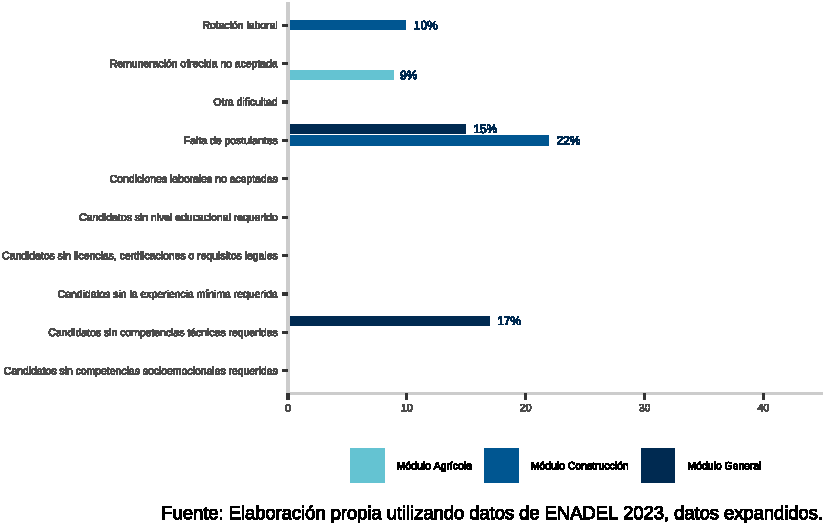
\includegraphics[width=1\textwidth,height=\textheight]{Reporte_files/figure-pdf/fig-dificultad-1.pdf}

}

\end{figure}%

\newpage

\subsection{Educación y experiencia}\label{educaciuxf3n-y-experiencia}

El 86,5\% de los cargos\footnote{Esta pregunta sólo se realiza para las
  ocupaciones señaladas en el módulo de ``Otros Cargos''.} consultados
tienen algún requisito de nivel educacional. La
Figura~\ref{fig-educ-tot} muestra la frecuencia con la que se solicita
cada nivel educacional como requisito.

\begin{figure}[H]

\caption{\label{fig-educ-tot}Frecuencia de requisitos educacionales
requeridos}

\centering{

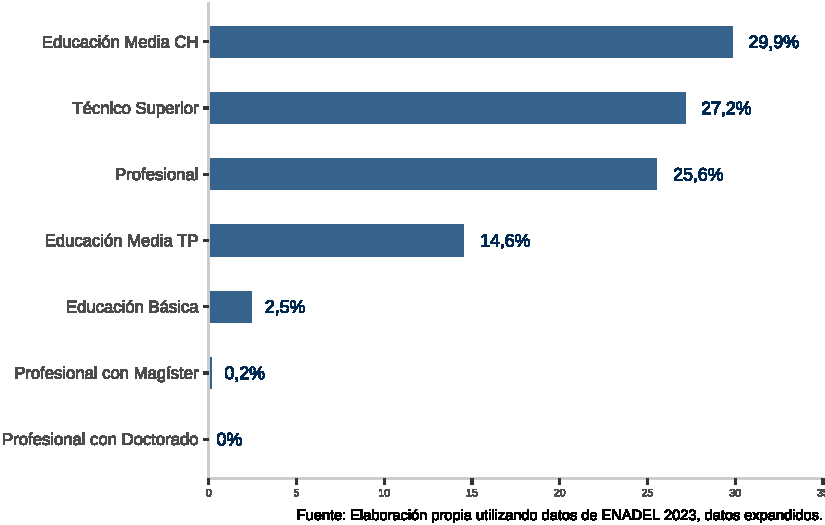
\includegraphics{Reporte_files/figure-pdf/fig-educ-tot-1.pdf}

}

\end{figure}%

Al consultar sobre experiencia requerida para el cargo, en el 33,8\% de
los casos se declara que el cargo no requiere experiencia. Para aquellas
ocupaciones donde si se señala experiencia laboral como uno de los
requisitos, el promedio total es de 2,6 años de experiencia (con un
error estándar de 0,12), sin haber mucha variación a través de los
distintos tamaños de empresa: se solicitan 2.8, 2.4 y 2.6 años en
promedio para empresas pequeñas, medianas y grandes, respectivamente.

\begin{table}

\caption{\label{tbl-exp_mean_sector}Experiencia laboral promedio
solicitada por sector de actividad económica.}

\centering{

\centering
\begin{tabular}{>{\raggedright\arraybackslash}p{9cm}>{\raggedright\arraybackslash}p{3cm}>{\raggedleft\arraybackslash}p{3cm}}
\toprule
Sector de Actividad Económica & \% que solicita experiencia & Experiencia promedio (años)\\
\midrule
Actividades financieras y de seguros & 78,6\% & 2,6\\
Transporte y almacenamiento & 74,4\% & 2,5\\
Información y comunicaciones & 72,8\% & 2,3\\
Actividades profesionales & 72\% & 3,4\\
Industria manufacturera & 70,1\% & 2,6\\
\addlinespace
Servicios administrativos y de apoyo & 68,7\% & 2,3\\
Actividades inmobiliarias & 68,4\% & 2,1\\
Construcción & 62,6\% & 3,0\\
Comercio & 59,8\% & 2,2\\
Silvoagropecuario & 59,3\% & 2,2\\
\addlinespace
Pesca y acuicultura & 55,8\% & 1,9\\
Administración pública & 55,1\% & 2,6\\
Alojamiento y de servicio de comidas & 54,3\% & 1,9\\
\bottomrule
\multicolumn{3}{l}{\rule{0pt}{1em}Fuente: Elaboración propia utilizando datos de ENADEL 2023, datos expandidos.}\\
\end{tabular}

}

\end{table}%

La Figura~\ref{fig-top_and_bottom} muestra a los tres sectores con mayor
y menor proporción de empresas que tienen requisitos de experiencia para
las nuevas contrataciones en los cargos consultados. Para aquellos
sectores que solicitan experiencia con más frecuencia, el promedio
supera los dos años, siendo ``Actividades financieras y de seguros'' el
sector que más solicita, con 2.6 años en promedio.

\begin{figure}[H]

\caption{\label{fig-top_and_bottom}Años de experiencia promedio para
sectores que solicitan más y menos experiencia}

\centering{

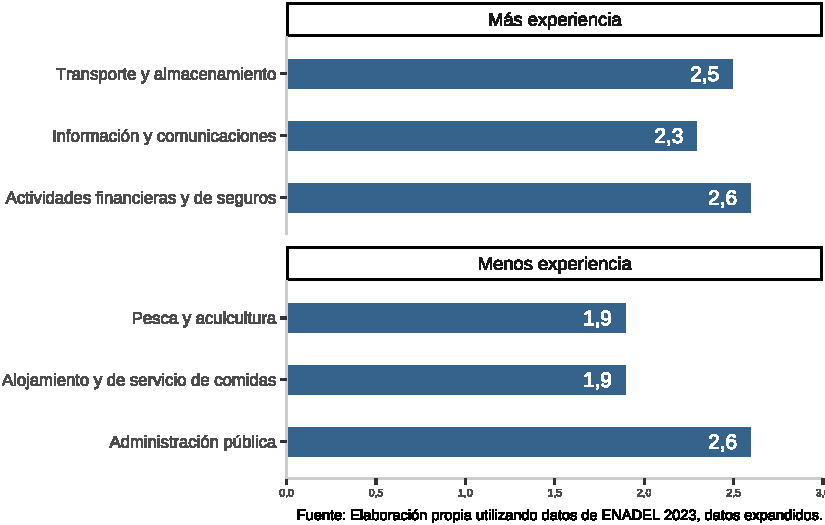
\includegraphics{Reporte_files/figure-pdf/fig-top_and_bottom-1.pdf}

}

\end{figure}%

Con respecto a la experiencia solicitada por sector de actividad
económica, los sectores de ``Pesca y acuicultura'' y de ``Alojamiento y
de servicio de comidas'' son los que requieren menos años de experiencia
(\text{1,9} años en promedio); mientras que ``Actividades
profesionales'' es el que más años de experiencia requiere, con
\text{3,4} años en promedio.

\subsection{Canales de reclutamiento}\label{canales-de-reclutamiento}

Frente a la pregunta \footnote{Esta pregunta sólo se realiza para las
  ocupaciones señaladas en el módulo de ``Otros Cargos''.}:

\emph{¿Nos puede indicar que canales o medios de contratación utilizó en
los procesos de reclutamiento y búsqueda de personas?}

La Tabla 18 muestra la proporción de cada uno de los canales
mencionados, tanto para el primer canal mencionado, como para el total.

\begin{table}

\caption{\label{tbl-canal}Canales de reclutamiento más utilizados,
ENADEL 2023}

\centering{

\centering
\begin{tabular}{>{\raggedright\arraybackslash}p{9cm}>{\raggedright\arraybackslash}p{3cm}>{\raggedright\arraybackslash}p{3cm}}
\toprule
Canal de reclutamiento & 1° Canal & Total\\
\midrule
Recomendaciones de trabajadores de la empresa u otros actores & 21\% & 21,3\%\\
Plataforma web de empleo pagada & 28,2\% & 20,2\%\\
Redes sociales & 13,3\% & 13,2\%\\
Redes personales del empleador & 8,8\% & 10,8\%\\
Plataforma web de empleo privada gratuita & 7\% & 8,6\%\\
\addlinespace
Oficina Municipal de Información Laboral & 5,8\% & 6,8\%\\
Avisos en la calle o banco de Curriculums & 2,6\% & 3,9\%\\
Diario o radio & 4\% & 3,6\%\\
Contratación de empresas de reclutamiento & 4,3\% & 3,5\%\\
Bolsa Nacional de Empleo & 2\% & 3\%\\
\addlinespace
Otro & 1,7\% & 2,8\%\\
Redes de profesionales, egresados o contacto con universidades & 1,3\% & 2,2\%\\
\bottomrule
\multicolumn{3}{l}{\rule{0pt}{1em}Fuente: Elaboración propia utilizando datos de ENADEL 2023, datos expandidos.}\\
\end{tabular}

}

\end{table}%

Considerando el total de respuestas (los tres canales mencionados), se
tiene que las principales vías de reclutamiento son ``Recomendaciones de
trabajadores de la empresa u otros actores'' con 21,3\% y ``Plataforma
web de empleo pagada'' con un 20,2\%. Los canales menos utilizados según
las menciones son, ``Redes de profesionales, egresados o contacto con
universidades'' con apenas un 2,2\%, y ``Bolsa Nacional de Empleo'', con
el 3\% .

\subsection{Conocimiento de instituciones y
programas}\label{conocimiento-de-instituciones-y-programas}

Frente a la pregunta: \emph{¿Conoce, y ha accedido a beneficios de las
siguientes instituciones o servicios públicos?}

SENCE SENCE se posiciona como la institución y/o servicio con más
conocimiento, con un 94,2\% de conocimiento, seguido de CORFO (85,6\%) y
OMIL (75,9\%). SENCE lidera el ranking de uso, con un 40,2\%, seguido
por las OMIL (34\%) y la BNE (17,4\%). Chile Valora es la institución
con menor conocimiento, con sólo un 36\% de los encuestados declarando
que lo conocen.

\begin{figure}[H]

\caption{\label{fig-conocimiento_1}Conocimiento sobre beneficios de
instituciones o servicios públicos, ENADEL 2023.}

\centering{

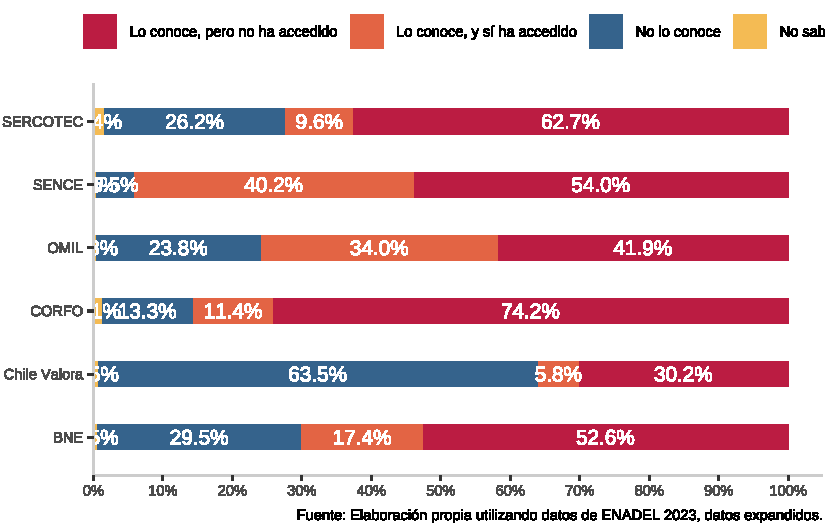
\includegraphics{Reporte_files/figure-pdf/fig-conocimiento_1-1.pdf}

}

\end{figure}%

Por otro lado, la frente a la pregunta: \emph{¿Conoce, y ha accedido a
beneficios de los siguientes programas o subsidios públicos?}

Los subsidios Subsidio al Empleo Joveny Bono Trabajo Mujer son los
programas con un mayor nivel de conocimiento (75,6\%y 69,9\%,
respectivamente), seguido por el programa FOSIS (57,5\%) y las FERIAS
LABORALES (56,7\%). Con respecto al nivel de uso, los programas de
subsidio también lideran, seguido de la FRANQUICIA TRIBUTARIA ( 24,2\%).

\begin{figure}[H]

\caption{\label{fig-conocimiento_2}Conocimiento sobre beneficios de
programas o subsidios públicos, ENADEL 2023.}

\centering{

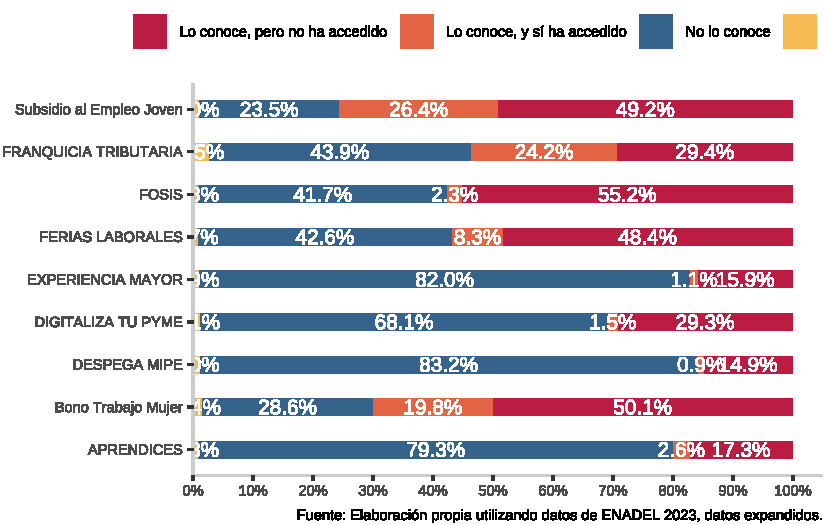
\includegraphics{Reporte_files/figure-pdf/fig-conocimiento_2-1.pdf}

}

\end{figure}%

La mayoría de los programas tienen un bajo nivel de conocimiento:
DESPEGA MIPE, EXPERIENCIA MAYOR y APRENDICES tienen tasas de
conocimiento inferiores al 19,9\%, y DIGITALIZA TU PYME de alrededor del
30,8\%.

\newpage

\subsection{Apéndice A: Ocupaciones de Difícil
Cobertura}\label{apuxe9ndice-a-ocupaciones-de-difuxedcil-cobertura}

\begin{longtable}{r>{\raggedright\arraybackslash}p{9cm}rl}

\caption{\label{tbl-vacantes_totales}}

\tabularnewline

\toprule
CIUO\_08 & Glosa & Vacantes & CV\\
\midrule
9211 & Obreros de explotaciones agrícolas & 15147 & 36,5\%\\
2423 & Especialistas en políticas y servicios de personal & 2459 & 100\%\\
9333 & Obreros de carga & 2381 & 42\%\\
7212 & Soldadores y oxicortadores & 2212 & 48,1\%\\
9321 & Empacadores manuales & 1930 & 76\%\\
\addlinespace
9112 & Auxiliares de aseo de oficinas, hoteles y otros establecimientos & 1864 & 23,9\%\\
7126 & Gásfiter e instaladores de tuberías & 1752 & 69,5\%\\
5414 & Guardias de seguridad & 1727 & 30,4\%\\
3113 & Técnicos en electricidad & 1572 & 65,2\%\\
8322 & Conductores de automóviles, taxis y camionetas & 1503 & 36,9\%\\
\addlinespace
4321 & Empleados encargados del control de abastecimiento e inventario & 1447 & 45,1\%\\
9412 & Ayudantes de cocina & 1428 & 45,5\%\\
2421 & Especialistas y asesores de gestión & 1191 & 94\%\\
5223 & Vendedores y asistentes de venta de tiendas, almacenes y puestos de mercado & 1086 & 37,1\%\\
8332 & Conductores de camiones pesados y de alto tonelaje & 997 & 26,1\%\\
\addlinespace
9329 & Obreros de la industria manufacturera no clasificados previamente & 970 & 51,3\%\\
7115 & Carpinteros de obra & 853 & 76,7\%\\
9212 & Obreros de explotaciones ganaderas & 811 & 70,4\%\\
5120 & Cocineros & 787 & 43,8\%\\
9621 & Mensajeros, estafetas, maleteros y repartidores de folletos y diarios a domicilio & 726 & 99,1\%\\
\addlinespace
8331 & Conductores de buses y trolebuses & 688 & 41,2\%\\
9622 & Auxiliares de mantenimiento (pequeñas reparaciones) & 678 & 97,5\%\\
2433 & Profesionales de ventas técnicas y médicas (excluyendo las TIC) & 662 & 69,1\%\\
5131 & Garzones de mesa & 633 & 45,2\%\\
7411 & Electricistas de obras & 630 & 80,6\%\\
\addlinespace
9411 & Cocineros de comida rápida & 618 & 58,8\%\\
2512 & Desarrolladores de software & 588 & 76,6\%\\
3512 & Técnicos en asistencia al usuario de tecnología de la información y las comunicaciones & 576 & 72,9\%\\
7515 & Catadores, clasificadores y controladores de calidad de alimentos y bebidas & 551 & 67,3\%\\
6111 & Agricultores y trabajadores calificados de cultivos extensivos & 542 & 66,4\%\\
\addlinespace
7412 & Mecánicos y ajustadores electricistas & 534 & 54,6\%\\
9122 & Limpiadores de vehículos & 510 & 69,7\%\\
7233 & Mecánicos y reparadores de máquinas agrícolas e industriales & 499 & 31,3\%\\
1221 & Directores, gerentes y administradores de comercialización & 494 & 88\%\\
8343 & Operadores de grúas y aparatos elevadores & 489 & 28,8\%\\
\addlinespace
7127 & Mecánicos de instalaciones de refrigeración y aire acondicionado & 466 & 96\%\\
9313 & Obreros de la construcción de edificios & 459 & 45\%\\
3221 & Técnicos y auxiliares paramédicos de enfermería & 450 & 96,2\%\\
2152 & Ingenieros electrónicos & 433 & 100\%\\
2221 & Enfermeros profesionales & 433 & 100\%\\
\addlinespace
5244 & Vendedores por internet y otros medios de comunicación & 413 & 100\%\\
3257 & Inspectores de la salud y técnicos en prevención de riesgos & 398 & 57,8\%\\
8344 & Operadores de autoelevadoras y montacargas & 395 & 44,8\%\\
7231 & Mecánicos y reparadores de vehículos de motor & 370 & 48,7\%\\
4110 & Trabajadores de tareas administrativas generales & 367 & 59,9\%\\
\addlinespace
2514 & Programadores de aplicaciones & 363 & 71,2\%\\
1323 & Directores, gerentes y administradores de empresas de construcción & 361 & 65,5\%\\
8142 & Operadores de máquinas para fabricar productos de material plástico & 359 & 56,4\%\\
5242 & Promotores de tiendas & 357 & 100\%\\
8143 & Operadores de máquinas para fabricar productos de papel & 353 & 91,3\%\\
\addlinespace
7422 & Instaladores y reparadores en tecnología de la información y las comunicaciones & 340 & 65,6\%\\
3322 & Representantes comerciales (excepto venta de productos y servicios industriales, farmacéuticos y de tecnologías de la información y las comunicaciones) & 316 & 80\%\\
3114 & Técnicos en electrónica & 304 & 52,2\%\\
5112 & Revisores y cobradores de los transportes públicos & 298 & 75,6\%\\
4225 & Empleados de informaciones, reclamos o sugerencias & 294 & 83,3\%\\
\addlinespace
4120 & Secretarios generales & 292 & 88\%\\
5246 & Vendedores de comidas al mostrador & 286 & 53,2\%\\
3313 & Técnicos y asistentes en contabilidad & 278 & 60,8\%\\
7223 & Reguladores y operarios de máquinas herramientas & 260 & 46\%\\
4226 & Recepcionistas (funciones generales) & 253 & 83,2\%\\
\addlinespace
3312 & Ejecutivos de préstamos y créditos & 226 & 66,9\%\\
9214 & Ayudantes de jardinería y horticultura & 225 & 78,4\%\\
5230 & Vendedores de entradas (entretenciones y eventos deportivos) y cajeros de comercio & 195 & 57,2\%\\
7112 & Albañiles & 185 & 53,2\%\\
2153 & Ingenieros en telecomunicaciones & 175 & 99,1\%\\
\addlinespace
7512 & Panaderos, pasteleros y confiteros & 171 & 31,2\%\\
6130 & Productores y trabajadores calificados de explotaciones agropecuarias mixtas & 161 & 64,4\%\\
3111 & Técnicos en ciencias físicas y químicas & 157 & 70,1\%\\
9334 & Reponedores de estanterías & 157 & 54,8\%\\
2411 & Contadores & 151 & 48,3\%\\
\addlinespace
5419 & Otro personal de los servicios de protección no clasificados previamente & 146 & 100\%\\
1330 & Directores, gerentes y administradores de servicios de tecnología de la información y las comunicaciones & 138 & 83,3\%\\
5245 & Bomberos de gasolineras & 138 & 51,9\%\\
7119 & Otros operarios de la construcción (obra gruesa) no clasificados previamente & 136 & 72,6\%\\
8341 & Operadores de maquinaria agrícola y forestal móvil & 133 & 43,4\%\\
\addlinespace
7541 & Buzos & 132 & 71,5\%\\
2242 & Químicos farmacéuticos & 129 & 71,4\%\\
2243 & Ingenieros en prevención de riesgos y otros profesionales de la seguridad e higiene laboral y ambiental & 129 & 40,5\%\\
7543 & Clasificadores, probadores de productos e inspectores de calidad (excluyendo alimentos y bebidas) & 129 & 84,6\%\\
1412 & Directores, gerentes y administradores de restaurantes & 127 & 68\%\\
\addlinespace
7421 & Mecánicos y reparadores en electrónica & 126 & 93,1\%\\
3323 & Agentes responsables de adquisiciones & 119 & 90,1\%\\
3521 & Técnicos de radiodifusión y grabación audiovisual & 117 & 100\%\\
2611 & Abogados & 115 & 93,5\%\\
5222 & Supervisores de locales comerciales, tiendas y almacenes & 114 & 78,4\%\\
\addlinespace
7511 & Carniceros y pescaderos & 108 & 51,9\%\\
8131 & Operadores de plantas y máquinas para fabricar productos químicos & 107 & 100\%\\
3115 & Técnicos en ingeniería mecánica & 105 & 57\%\\
4224 & Recepcionistas de hoteles & 99 & 60,1\%\\
7544 & Fumigadores y otros controladores de plagas y malezas & 97 & 79,6\%\\
\addlinespace
3142 & Técnicos agropecuarios (incluyendo acuícolas) & 94 & 66,7\%\\
2142 & Ingenieros civiles, ingenieros en construcción y constructores civiles & 92 & 38,3\%\\
2511 & Analistas de sistemas & 91 & 90,9\%\\
9213 & Obreros de explotaciones agropecuarias & 90 & 79,8\%\\
2513 & Desarrolladores Web y multimedia & 83 & 100\%\\
\addlinespace
2519 & Otros desarrolladores y analistas de software y multimedia no clasificados previamente & 83 & 100\%\\
4132 & Digitadores de datos & 82 & 69,7\%\\
7413 & Instaladores y reparadores de líneas eléctricas & 82 & 82,9\%\\
8342 & Operadores de máquinas de movimiento de tierras & 79 & 36,2\%\\
7214 & Montadores de estructuras metálicas & 78 & 48\%\\
\addlinespace
2434 & Profesionales de ventas de tecnología de la información y las comunicaciones (TIC) & 74 & 70,7\%\\
2341 & Profesores de educación básica & 73 & 100\%\\
1420 & Directores, gerentes y administradores de comercios al por mayor y al por menor & 71 & 59,6\%\\
8183 & Operadores de máquinas de embalaje, embotellamiento y etiquetado & 70 & 80,2\%\\
2145 & Ingenieros químicos & 68 & 100\%\\
\addlinespace
2529 & Otros especialistas en bases de datos y en redes de computadores no clasificados previamente & 65 & 71,6\%\\
3123 & Supervisores de la construcción & 61 & 44,8\%\\
2431 & Profesionales de la publicidad y la comercialización & 60 & 97,5\%\\
8172 & Operadores de instalaciones de procesamiento de la madera & 59 & 57,7\%\\
9611 & Recolectores de basura y material reciclable & 59 & 100\%\\
\addlinespace
2230 & Veterinarios & 58 & 76,8\%\\
1212 & Directores, gerentes y administradores de recursos humanos & 56 & 77,9\%\\
3522 & Técnicos de ingeniería de las telecomunicaciones & 56 & 72,3\%\\
2144 & Ingenieros mecánicos & 55 & 51,1\%\\
2165 & Cartógrafos y agrimensores & 54 & 100\%\\
\addlinespace
7132 & Barnizadores y pulverizadores de productos manufacturados & 52 & 70,7\%\\
8160 & Operadores de máquinas para elaborar alimentos, bebidas y cigarrillos & 52 & 61,4\%\\
1321 & Directores, gerentes y administradores de industrias manufactureras & 51 & 54,2\%\\
3331 & Agentes de aduana & 46 & 63,9\%\\
3343 & Secretarios administrativos y ejecutivos & 45 & 49,6\%\\
\addlinespace
1324 & Directores, gerentes y administradores de empresas de abastecimiento, almacenamiento y distribución & 43 & 62,3\%\\
8350 & Tripulantes de cubierta de barco & 43 & 52,9\%\\
1311 & Directores, gerentes y administradores de producción y operaciones agropecuarias y de silvicultura & 37 & 76,7\%\\
3112 & Técnicos en construcción y topógrafos & 37 & 58,4\%\\
8321 & Conductores de motocicletas & 36 & 100\%\\
\addlinespace
9629 & Otras ocupaciones elementales no clasificadas previamente & 35 & 71,9\%\\
3240 & Técnicos y asistentes veterinarios & 34 & 86,7\%\\
2522 & Administradores de sistemas & 33 & 99,1\%\\
3434 & Chefs & 32 & 61,4\%\\
4416 & Empleados y asistentes de recursos humanos & 32 & 55,4\%\\
\addlinespace
8141 & Operadores de máquinas para fabricar productos de caucho & 32 & 100\%\\
8151 & Operadores de máquinas de preparación de fibras, hilado y devanado & 32 & 100\%\\
3131 & Operadores de instalaciones de producción de energía & 31 & 100\%\\
7122 & Instaladores de parqué, cerámicas, baldosas y alfombras & 31 & 76,2\%\\
1211 & Directores, gerentes y administradores de finanzas & 30 & 58,7\%\\
\addlinespace
6113 & Agricultores y trabajadores calificados de huertas, invernaderos, viveros y jardines & 30 & 70,7\%\\
7111 & Constructores de casas & 30 & 65,3\%\\
4313 & Empleados encargados de las nóminas o registros de remuneraciones & 29 & 61,6\%\\
5243 & Representantes de ventas de puerta a puerta (venta a hogares) & 29 & 67,7\%\\
2163 & Diseñadores de productos y de vestuario & 28 & 62,3\%\\
\addlinespace
2641 & Autores y otros escritores & 28 & 100\%\\
3143 & Técnicos forestales & 28 & 100\%\\
5132 & Bármanes & 28 & 46,2\%\\
6221 & Trabajadores de explotaciones de acuicultura & 27 & 69,6\%\\
7323 & Encuadernadores & 27 & 100\%\\
\addlinespace
9215 & Obreros forestales & 27 & 100\%\\
7322 & Impresores & 26 & 83,5\%\\
2413 & Analistas financieros & 24 & 69,9\%\\
8181 & Operadores de instalaciones de vidriería y cerámica & 24 & 100\%\\
9216 & Obreros de pesca y acuicultura & 24 & 100\%\\
\addlinespace
3439 & Otros técnicos en actividades culturales y artísticas no clasificados previamente & 23 & 100\%\\
2141 & Ingenieros industriales y de producción & 22 & 69,6\%\\
2166 & Diseñadores gráficos y de multimedia & 22 & 69,1\%\\
7121 & Instaladores o reparadores de techos & 22 & 100\%\\
7213 & Chapistas y caldereros & 22 & 100\%\\
\addlinespace
6112 & Agricultores y trabajadores calificados de plantaciones de árboles y arbustos & 20 & 58,2\%\\
3351 & Inspectores de aduana & 19 & 100\%\\
3513 & Técnicos en redes y sistemas de computadores & 19 & 65,8\%\\
3334 & Agentes inmobiliarios & 18 & 85,2\%\\
7522 & Ebanistas y mueblistas & 18 & 100\%\\
\addlinespace
2432 & Profesionales de las relaciones públicas & 17 & 56,8\%\\
5163 & Personal de pompas fúnebres y embalsamadores & 17 & 100\%\\
7523 & Operadores y reguladores de máquinas para trabajar la madera & 17 & 71\%\\
3151 & Oficiales maquinistas en navegación & 16 & 80,3\%\\
3341 & Supervisores de oficina & 16 & 79\%\\
\addlinespace
5249 & Otros vendedores no clasificados previamente & 16 & 76,2\%\\
1213 & Directores, gerentes y administradores de políticas empresariales y planificación & 15 & 100\%\\
3411 & Técnicos de los servicios jurídicos & 15 & 69,4\%\\
4222 & Empleados de centros de llamadas de informaciones & 15 & 100\%\\
4323 & Empleados de servicios de transporte & 14 & 57,9\%\\
\addlinespace
1411 & Directores, gerentes y administradores de hoteles & 13 & 100\%\\
2143 & Ingenieros medioambientales & 13 & 69,6\%\\
8219 & Ensambladores no clasificados previamente & 13 & 100\%\\
9510 & Trabajadores ambulantes de servicios & 13 & 100\%\\
2635 & Profesionales del trabajo social & 12 & 77,9\%\\
\addlinespace
6210 & Trabajadores forestales calificados & 12 & 100\%\\
2132 & Agrónomos y profesionales del ámbito forestal y pesquero & 11 & 100\%\\
2149 & Otros ingenieros no clasificados previamente & 10 & 100\%\\
7542 & Dinamiteros y pegadores & 10 & 100\%\\
8311 & Maquinistas de locomotoras & 10 & 100\%\\
\addlinespace
1112 & Personal directivo de la administración pública & 8 & 72,4\%\\
3152 & Capitanes y oficiales de cubierta & 8 & 60,5\%\\
9123 & Limpiadores de ventanas & 8 & 100\%\\
2131 & Biólogos, botánicos, zoólogos, genetistas y farmacólogos & 7 & 100\%\\
2248 & Terapeutas ocupacionales & 7 & 100\%\\
\addlinespace
2634 & Psicólogos & 7 & 100\%\\
3118 & Delineantes y dibujantes técnicos & 7 & 100\%\\
3412 & Técnicos en trabajo social & 7 & 100\%\\
7123 & Yeseros, estucadores y revocadores & 7 & 100\%\\
5164 & Cuidadores de animales & 6 & 100\%\\
\addlinespace
2151 & Ingenieros eléctricos & 5 & 100\%\\
2211 & Médicos generales & 5 & 100\%\\
2642 & Periodistas & 5 & 100\%\\
4221 & Empleados de agencias de viajes & 5 & 100\%\\
4311 & Auxiliares y ayudantes de registros de contabilidad y cálculo de costos & 5 & 56,9\%\\
\addlinespace
7114 & Operarios en cemento armado & 5 & 100\%\\
1120 & Directores y gerentes generales de empresas & 4 & 72,3\%\\
3354 & Agentes de servicios de tramitación y entrega de licencias y permisos & 4 & 94,1\%\\
3511 & Técnicos en operaciones de tecnología de la información y las comunicaciones & 4 & 100\%\\
5411 & Bomberos & 4 & 100\%\\
\addlinespace
8157 & Operadores de máquinas de lavanderías & 4 & 100\%\\
2164 & Urbanistas e ingenieros de transporte y tránsito & 3 & 100\%\\
3514 & Técnicos de la Web & 3 & 100\%\\
5151 & Supervisores de mantenimiento y limpieza en oficinas, hoteles y otros establecimientos & 3 & 70,7\%\\
9121 & Lavanderos y planchadores manuales & 3 & 100\%\\
\addlinespace
2632 & Sociólogos, antropólogos, geógrafos y arqueólogos & 2 & 100\%\\
3122 & Supervisores de industrias manufactureras & 2 & 100\%\\
4415 & Empleados administrativos de archivos & 2 & 100\%\\
9612 & Clasificadores de desechos & 2 & 100\%\\
1344 & Directores, gerentes y administradores de servicios de bienestar social & 1 & 100\%\\
\addlinespace
2161 & Arquitectos & 1 & 100\%\\
4223 & Telefonistas & 1 & 99,3\%\\
7533 & Costureros y bordadores & 1 & 100\%\\
\bottomrule
\multicolumn{4}{l}{\rule{0pt}{1em}Fuente: Elaboración propia utilizando datos de ENADEL 2023, datos expandidos.}\\

\end{longtable}

\newpage
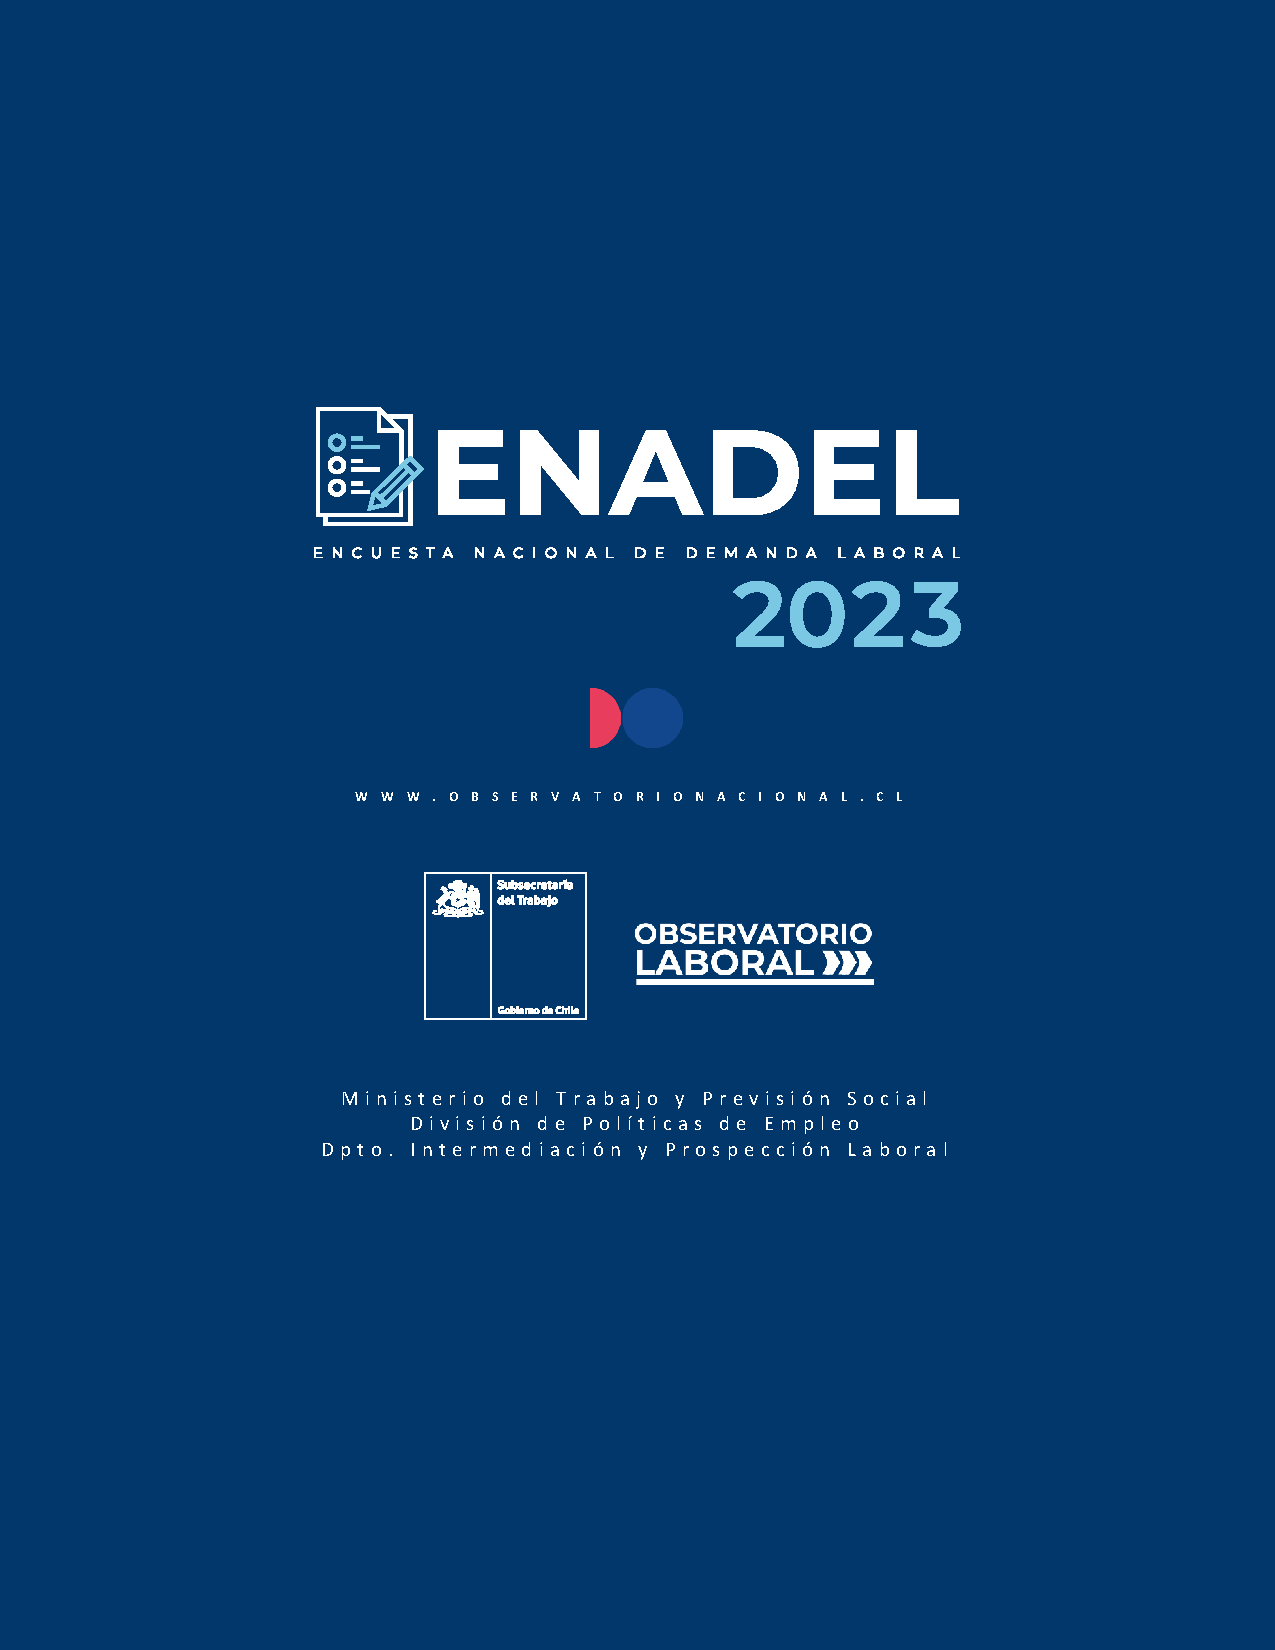
\includepdf[pages=-]{../Quarto/Portada/Portadas-Enadel-2023-5.pdf}




\end{document}
